\chapter{Results}

In this chapter, we present the results of the literature survey based on the literature repository that we constructed in Chapter 3. The literature repository is stored in the author's local computer and management by a reference management software Zotero. We extract and organize the results based on our evaluation matrices but in different categories \textcolor{red}{unclear reference of different categories} of studies. In the following subsections, we first present the overview and comparison of the literature in our paper repository, and then we summarize and highlight the most impact research in each category. Finally, we summarize findings from our review.

\section{Overview}

\textbf{Year Distribution:} Earlier research on expertise focus the cognitive science of how experts think and act. Though several directional \cite{mcdonald1998just, mcdonald2000expertise, mockus2002expertise} emerged around 2000, most follow-up studies were published in the following decade. Especially since the popularity of machine learning techniques, and to the best our knowledge, after the first study \cite{Anvik2006who} applied machine learning techniques in locating expertise for bug report assignment,  there are more studies applies statistical models via machine learning to analyze human factors in software engineering \cite{xu2016predicting, ye2014learning}. In our paper repository, most studies were published in the 2010s (See Figure \ref{yeardis}).

There are 20 journal publications and 28 conference publications respectively in venues of CSCW, Software Engineering and a few in HCI. Software Engineering has the most published papers in this repository (28 out of 48).

\pgfplotstableread[row sep=\\,col sep=&]{
    Year & Count \\
    1981 & 1 \\
    1982 & 0 \\
    1983 & 0 \\
    1984 & 1 \\
    1985 & 0 \\
    1986 & 0 \\
    1987 & 0 \\
    1988 & 1 \\
    1989 & 0 \\
    1990 & 0 \\
    1991 & 1 \\
    1992 & 0 \\
    1993 & 0 \\
    1994 & 2 \\
    1995 & 0 \\
    1996 & 0 \\
    1997 & 1 \\
    1998 & 1 \\
    1999 & 0 \\
    2000 & 1 \\
    2001 & 0 \\
    2002 & 2 \\
    2003 & 0 \\
    2004 & 0 \\
    2005 & 0 \\
    2006 & 1 \\
    2007 & 3 \\
    2008 & 2 \\
    2009 & 1 \\
    2010 & 2 \\
    2011 & 1 \\
    2012 & 5 \\
    2013 & 3 \\
    2014 & 6 \\
    2015 & 0 \\
    2016 & 9 \\
    2017 & 3 \\
    }\yeardata
\begin{figure}

    \begin{tikzpicture}
        \begin{axis}[
                ybar,
                width=\textwidth,
                height=.5\textwidth,
                nodes near coords,
                symbolic x coords={1981,1982,1983,1984,1985,1986,1987,1988,1989,1990,1991,1992,1993,1994,1995,1996,1997,1998,1999,2000,2001,2002,2003,2004,2005,2006,2007,2008,2009,2010,2011,2012,2013,2014,2015,2016,2017},
                % xtick=data,
                xtick pos=bottom,
                ytick pos=left,
                ylabel={Count},
            ]
            \addplot table[x=Year,y=Count]{\yeardata};
        \end{axis}
    \end{tikzpicture}
    \caption{Publication Year Distribution of Papers in Literature Repository}
    \label{yeardis}
\end{figure}

\textbf{Impact/Citation Count:} The average citation count of these studies is 99.4, and there are 10 studies have over one hundred citations. Hence, we argue that studies in our literature repository represent the research on expertise locations and automating this process.

\textbf{Research Type:} There are 23 empirical studies, 18 case studies, and 7 conceptual studies. Noticeably, one study conducted observation in the field to build a ground theory for expertise location method in software engineering practice \cite{mcdonald1998just}. Among these studies, 23 of them only use quantitative approaches to analyze their collected data, and 11 studies only apply qualitative approaches in their studies. Further, 7 studies apply the mixed-method to identify the evidence to support their conclusions. According to our literature repository, we found there is a variety of research methods based on their research focuses. Studies that mine historical artifacts usually apply quantitative methods to model expertise \cite{Anvik2006who, minto2007recommending, mockus2002expertise, vasilescu2014social}, and studies explore the expert characteristics and sharing expertise apply qualitative research method \cite{chen2016towards, koenemann1991expert, ley2014information, waterson1997dynamics}.

\section{Primary Studies}

In the final literature repository, we read the paper in full and then extract necessary data from each paper. Therefore, in the end, we identified these studies as primary (see Table \ref{tab:primaryStudies}) based on their focused expertise domains and correspondence to our research questions.

\begin{table}[tbp]
\centering
\begin{tabular}{llll} 
\hline
\textbf{Year}           & \textbf{Reference}          & \textbf{Year}           & \textbf{Reference} \\ \hline
\citeyear{MCKEITHEN1981307} & \citeauthor{MCKEITHEN1981307} \cite{MCKEITHEN1981307} 
& \citeyear{Dabbish2012social} &  \citeauthor{Dabbish2012social} \cite{Dabbish2012social} \\

\citeyear{soloway1984empirical} & \citeauthor{soloway1984empirical} \cite{soloway1984empirical}
& \citeyear{hanrahan2012modeling} &  \citeauthor{hanrahan2012modeling} \cite{hanrahan2012modeling} \\

\citeyear{pinto1988providing} & \citeauthor{pinto1988providing} \cite{pinto1988providing}
& \citeyear{servant2012whosefault} &  \citeauthor{servant2012whosefault} \cite{servant2012whosefault} \\

\citeyear{koenemann1991expert} & \citeauthor{koenemann1991expert} \cite{koenemann1991expert}
& \citeyear{maalej2013patterns} &  \citeauthor{maalej2013patterns} \cite{maalej2013patterns} \\

\citeyear{davies1994knowledge} & \citeauthor{davies1994knowledge} \cite{davies1994knowledge}
& \citeyear{ackerman2013sharing} &  \citeauthor{ackerman2013sharing} \cite{ackerman2013sharing} \\

\citeyear{stanislaw1994note} &  \citeauthor{stanislaw1994note} \cite{stanislaw1994note} 
& \citeyear{yarosh2013need} &  \citeauthor{yarosh2013need} \cite{yarosh2013need} \\

\citeyear{waterson1997dynamics} &  \citeauthor{waterson1997dynamics} \cite{waterson1997dynamics} 
& \citeyear{fritz2014degree} & \citeauthor{fritz2014degree} \cite{fritz2014degree} \\

\citeyear{mcdonald1998just} &  \citeauthor{mcdonald1998just} \cite{mcdonald1998just} 
& \citeyear{vasilescu2014social} &  \citeauthor{vasilescu2014social} \cite{vasilescu2014social} \\

\citeyear{mcdonald2000expertise} &  \citeauthor{mcdonald2000expertise} \cite{mcdonald2000expertise} 
& \citeyear{maalej2014comprehension} &  \citeauthor{maalej2014comprehension} \cite{maalej2014comprehension} \\

\citeyear{mockus2002expertise} &  \citeauthor{mockus2002expertise} \cite{mockus2002expertise} 
& \citeyear{ye2014learning} &  \citeauthor{ye2014learning} \cite{ye2014learning} \\

\citeyear{nardi2002integrating} &  \citeauthor{nardi2002integrating} \cite{nardi2002integrating} 
& \citeyear{ley2014information} &  \citeauthor{ley2014information} \cite{ley2014information} \\

\citeyear{chevalier2003web} &  \citeauthor{chevalier2003web} \cite{chevalier2003web} 
& \citeyear{bergersen2014construction} &  \citeauthor{bergersen2014construction} \cite{bergersen2014construction} \\

\citeyear{Anvik2006who} &  \citeauthor{Anvik2006who} \cite{Anvik2006who}
& \citeyear{chan2016improving} &  \citeauthor{chan2016improving} \cite{chan2016improving} \\

\citeyear{minto2007recommending} &  \citeauthor{minto2007recommending} \cite{minto2007recommending} 
& \citeyear{xu2016predicting} &  \citeauthor{xu2016predicting} \cite{xu2016predicting} \\

\citeyear{anvik2007determining} &  \citeauthor{anvik2007determining} \cite{anvik2007determining} 
& \citeyear{thongtanunam2016revisiting} &  \citeauthor{thongtanunam2016revisiting} \cite{thongtanunam2016revisiting} \\

\citeyear{Reichling2007} &  \citeauthor{Reichling2007} \cite{Reichling2007} 
& \citeyear{yu2016reviewer} &  \citeauthor{yu2016reviewer} \cite{yu2016reviewer} \\

\citeyear{yang2008social} &  \citeauthor{yang2008social} \cite{yang2008social} 
& \citeyear{costa2016tipmerge} &  \citeauthor{costa2016tipmerge} \cite{costa2016tipmerge} \\

\citeyear{schuler2008mining} &  \citeauthor{schuler2008mining} \cite{schuler2008mining}
& \citeyear{rahman2016correct} &  \citeauthor{rahman2016correct} \cite{rahman2016correct} \\

\citeyear{lin2009smallblue} &  \citeauthor{lin2009smallblue} \cite{lin2009smallblue} 
& \citeyear{hannebauer2016automatically} &  \citeauthor{hannebauer2016automatically} \cite{hannebauer2016automatically} \\

\citeyear{klas2010transparent} &  \citeauthor{klas2010transparent} \cite{klas2010transparent}
& \citeyear{hiring2016sarma} &  \citeauthor{hiring2016sarma} \cite{hiring2016sarma} \\

\citeyear{fritz2010degree} &  \citeauthor{fritz2010degree} \cite{fritz2010degree} 
& \citeyear{greene2016cvexplorer} &  \citeauthor{greene2016cvexplorer} \cite{greene2016cvexplorer} \\

\citeyear{gottipati2011finding} &  \citeauthor{gottipati2011finding} \cite{gottipati2011finding}
& \citeyear{lin2017improving} &  \citeauthor{lin2017improving} \cite{lin2017improving} \\

\citeyear{pipek2012bridging} &  \citeauthor{pipek2012bridging} \cite{pipek2012bridging} 
& \citeyear{saxena2017know} &  \citeauthor{saxena2017know} \cite{saxena2017know} \\

\citeyear{bednarik2012expertise} &  \citeauthor{bednarik2012expertise} \cite{bednarik2012expertise}
& \citeyear{wang2017recommending} &  \citeauthor{wang2017recommending} \cite{wang2017recommending} \\

\hline
\end{tabular}
\caption{Primary Studies in the Literature Repository}
\label{tab:primaryStudies}
\end{table}

In our literature repository, we identify two categories of expertise research: 1) identify the characteristics of experts, 2) locating experts.

% types of research
\pgfplotstableread[row sep=\\,col sep=&]{
    Type & Count \\
    Characteristics & 8 \\
    Manual & 5 \\
    Historic & 18 \\
    Sharing & 8 \\
    Network & 2 \\
    Others & 7 \\
    }\typedata
\begin{figure}

    \begin{tikzpicture}
        \begin{axis}[
                ybar,
                width=\textwidth,
                height=.5\textwidth,
                nodes near coords,
                symbolic x coords={Characteristics, Manual, Historic, Sharing, Network, Others},
                bar width = 40,
                xtick=data,
                xtick pos=bottom,
                ytick pos=left,
                ylabel={Count},
                xticklabel style = {font=\tiny},
                xticklabels={
                    Expert Characteristics,
                    Manual Location,
                    Mining Historical,
                    Sharing Content,
                    Sharing Network,
                    Others,
                },
            ]
            \addplot table[x=Type,y=Count]{\typedata};
        \end{axis}
    \end{tikzpicture}
    \caption{Publication Category Distribution of Papers in Literature Repository}
    \label{typedis}
\end{figure}

There are several early studies and a few recent studies intend to empirically identify the characteristics of experts in software engineering by monitoring their performance, see Table \ref{tab:expertCharacteristics}. There are studies explore the information processing ability of experts \cite{MCKEITHEN1981307}, the strategies that experts adopted in programming comprehension \cite{koenemann1991expert}, and validation expertise via monitoring experts performance \cite{davies1994knowledge, bergersen2014construction}.

\begin{table}[htbp]
\centering
\small
\settowidth\tymin{\textbf{Reference}}
\begin{tabulary}{\textwidth}{LLLL}
\hline
\textbf{Year}           & \textbf{Reference}          & \textbf{Approach}           & \textbf{Findings} \\ \hline
\citeyear{MCKEITHEN1981307} & \citeauthor{MCKEITHEN1981307}\cite{MCKEITHEN1981307} & Empirical Study & Experts in programming perform better in retrieving and recalling related information; experts' knowledge representations are similar.\\ \hline

\citeyear{soloway1984empirical} & \citeauthor{soloway1984empirical}\cite{soloway1984empirical} & Empirical Study & Empirically identified two types of knowledge in programming: plans and rules, which are heavily related to mind simulation and information processing. \\ \hline

\citeyear{koenemann1991expert} & \citeauthor{koenemann1991expert}\cite{koenemann1991expert} & Empirical Study & When understanding the program, experts search for relevant information in the code, and only employ a bottom-up strategy for entire program comprehension when their hypothesis failed.\\ \hline

\citeyear{davies1994knowledge} &\citeauthor{davies1994knowledge}\cite{davies1994knowledge} & Empirical Study & As the expertise growth for programming developers from lower to higher, when given a programming task, their reaction time and the number of errors made tend to be lower comparing to novices.\\ \hline

\citeyear{stanislaw1994note} &\citeauthor{stanislaw1994note}\cite{stanislaw1994note} & Empirical Study & Employ time factor, time of complete the programming task, and multitasking ability, the variety of programming skills such as the number of programming language known, to quantitatively measure expertise.\\\hline

\citeyear{maalej2014comprehension} & \citeauthor{maalej2014comprehension}\cite{maalej2014comprehension} & Case Study & Programmers comprehension strategies depends on the context, and they would avoid to understand whenever possible, similar to work of \citeauthor{koenemann1991expert}.\\\hline

\citeyear{bergersen2014construction} &\citeauthor{bergersen2014construction}\cite{bergersen2014construction} & Empirical Study & \citeauthor{bergersen2014construction} build testing model to systematically measure and valid the expertise level of programmers in Java. It validates expertise through the quality of answers and responsive time in series of programming tests, and also self-reported data of the experience and programming motivation.\\ \hline

\end{tabulary}
\caption{Primary Studies for Expert Characteristics}
\label{tab:expertCharacteristics}
\end{table}

% \begin{center}
\begin{table}[htbp]
\centering
\small
\settowidth\tymin{\textbf{Evaluation}}
\begin{tabulary}{\textwidth}{LLLLL}
\hline
\textbf{Year}           & \textbf{Reference}          & \textbf{Approach}           & \textbf{Findings}  & \textbf{Future Work}\\ \hline
\citeyear{waterson1997dynamics} & \citeauthor{waterson1997dynamics}\cite{waterson1997dynamics} & Case study: visited an IT company several times and conduct an interview-based qualitative study with key personnel in the organization & They identified the manual knowledge sharing network structure in a software development team. & Technology can be applied to the knowledge sharing process in the software development. Purpose a need of conducting case studies upon the different size of organizations to validate their structure. \\ \hline
\citeyear{mcdonald1998just} & \citeauthor{mcdonald1998just}\cite{mcdonald1998just} & Field study: conducted a field study in midsize IT company. & They found three major heuristics to locate expertise in software development practice: everyday experts, through an expertise concierge and mining historical artifacts. & Automated systems are needed to support situations in expertise location process such as the escalation behavior. \\\hline
\citeyear{pipek2012bridging} & \citeauthor{pipek2012bridging}\cite{pipek2012bridging} & Case study: longitudinal case studies in three organizations and summarize the frameworks for designing technologies for supporting expertise and knowledge management. & In expertise sharing of organizations, practice leads to technologies innovation. While integrating new tech, the new design should not disrupt the current ecosystem. & Follow the heuristics and carefully design new technologies for supporting expertise location and sharing activities. \\\hline
\citeyear{yarosh2013need} & \citeauthor{yarosh2013need}\cite{yarosh2013need} & Case study: They conducted a diary, and then interview study on professional software developers & They explore the expertise location practice, and they found in most cases (76\%) asking a colleague is the common practice to solve a problem, and tools are not helpful. & Time issue in the expertise (help) location activity. They found 15\% of the tasks involved in help-finding remained unsolved for longer than two weeks. \\\hline
\citeyear{thongtanunam2016revisiting} & \citeauthor{thongtanunam2016revisiting}\cite{thongtanunam2016revisiting} & Case Study: observe the code reviews of six software systems in the field & Majority of reviewers only contribute to one module on the system, and code reviewers with more reviewing experience are more significant in reducing the defects rather than with code authorship. & Future studies should majorly rely on using code review experience to determine best experts for reviewing the code.\\ \hline
\end{tabulary}
\caption{Primary Studies for Manual Location Approaches}
\label{tab:manual}
\end{table}
% \end{center}'

There are several studies investigated the practice of expertise location in software engineering, focusing on the common practice that manually locates experts (see Table \ref{tab:manual}). There is a study identifies the expertise sharing network structure in software development organizations \cite{waterson1997dynamics}. Moreover, there is a study identifies a set of practical strategies for locating expertise, which provides heuristics for automated expertise location systems \cite{mcdonald1998just}. Finally, there is a recent study that revisited the practices of expertise location in software organizations but found asking colleague is the most common practice, and automated location tools are hardly used \cite{yarosh2013need}.

\begin{sidewaystable}
\centering
\scriptsize
\settowidth\tymin{\textbf{Evaluation}}
\begin{tabulary}{\textwidth}{|LLLLLL|}
\hline
\textbf{Year}           & \textbf{Reference}          & \textbf{Domain}  &\textbf{Approach}  & \textbf{Evaluation}  & \textbf{Future Work}\\ \hline
\citeyear{mcdonald2000expertise} & \citeauthor{mcdonald2000expertise}\cite{mcdonald2000expertise} & Problem Casebase & Analyzing task similarity to find best expert for the current problem & Not applicable & Empirical study with developers.\\ \hline
\citeyear{mockus2002expertise} & \citeauthor{mockus2002expertise}\cite{mockus2002expertise} & Activity unit (Experience Atoms) & Accumulate the experience on historical artifacts to determine expertise & Usability test & Use time for completion to evaluate the expertise required for task; ``quantitative resume'' for developer.\\ \hline
\citeyear{Anvik2006who} & \citeauthor{Anvik2006who}\cite{Anvik2006who} & Bug report & Analyzing the Bug Report similarity and use machine learning techniques to recommend developers & Precision and recall & Empirical study with developers, additional source of information.\\ \hline
\citeyear{minto2007recommending} & \citeauthor{minto2007recommending}\cite{minto2007recommending} & Changes in historical artifacts & Apply file dependency and authorship matrix to produce expertise matrix, and finally support experts communication by locating expertise of task & Precision and recall & Empirical study with developers\\ \hline
\citeyear{anvik2007determining} & \citeauthor{anvik2007determining}\cite{anvik2007determining} & Bug Report & Empirically evaluate the expertise location approaches for bug report assignment: mining code artifacts and ``bug network''. & Precision and recall & Looking for approaches other than precision and recall to evaluate the expertise location system\\ \hline
\citeyear{Reichling2007} & \citeauthor{Reichling2007}\cite{Reichling2007} & Support Expertise Sharing & Aggregation of feedback for previous work, similarity of previous tasks and personal information. & Not applicable & Suggestion for applying technology in expertise sharing activities\\ \hline
\citeyear{schuler2008mining} & \citeauthor{schuler2008mining}\cite{schuler2008mining} & Code Artifacts & Measure expertise based on code usage data (calling) & Not applicable & Improving precision, combining with conventional authorship model, combining with task and bug reports, explore the relation between expertise and quality of work\\ \hline
\citeyear{servant2012whosefault} & \citeauthor{servant2012whosefault}\cite{servant2012whosefault} & Fault Localization & Aggregate the test cases results execution results with code modification history, and then generate the fault-to-developer assignment. & Empirically compare the WhoseFault with historical ground truth, naive methods, and other automated techniques. & Expand the WhoseFault tool with additional subjects and test cases, and also apply different mapping techniques for fault-to-developer assignment. \\\hline
\citeyear{maalej2013patterns} & \citeauthor{maalej2013patterns}\cite{maalej2013patterns} & API Documentation & List a taxonomy of knowledge type in API documentation through a four steps mix-method approach. & Case Study on two programming languages & Systematically identify the knowledge types in documentation rather than empirically. Address the gap between information seekers and providers.\\\hline
\citeyear{ye2014learning} & \citeauthor{ye2014learning}\cite{ye2014learning} & Bug Report & Employ machine learning techniques to aggregate data such as program classes name similarity and bug fixing history, and generate a list of files which are relevant to the bug. & Precision based evaluation metrics & Additional data source such as code authorship, and empirical evaluation with other projects.\\\hline
\citeyear{fritz2014degree} & \citeauthor{fritz2014degree}\cite{fritz2014degree} & Code Artifacts & Apply the Degree-of-Knowledge model to assess the expertise of a developer depending on her interaction with IDEs and code authorship (modification history) & Case Study with developers at three sites by applying the model to find experts. & Application in bug finding. Longitudinal studies with developers. Additional data source such as documentation. \\\hline
\citeyear{rahman2016correct} & \citeauthor{rahman2016correct}\cite{rahman2016correct} & Code Review & Determine code reviewer by code authorship and also experience with the collaboration model such as pull-request model on \textsc{GitHub}. &  Precision and recall, comparison with existing systems & Handling concurrent recommendation request\\\hline
\citeyear{greene2016cvexplorer} & \citeauthor{greene2016cvexplorer}\cite{greene2016cvexplorer} & Developer Profile & Retrieve developer related tags from \textsc{GitHub} activity history & Preliminary case study in two company hiring process. & Additional data source, longitudinal study in software practice, and evaluate the tool accuracy with manual extraction. \\\hline
\citeyear{costa2016tipmerge} & \citeauthor{costa2016tipmerge}\cite{costa2016tipmerge} & Merging Conflicts & Past experience of developers over different branches, and also the dependencies of modified files. & Empirical study uses historical data and compares with the actual person performed merge. & Integrate with more other algorithms, analyze in finer grain level, evaluate the project with other projects.\\\hline
\citeyear{lin2017improving} & \citeauthor{lin2017improving}\cite{lin2017improving} & Source Code Knowledge & Retrieve code-specific knowledge such API entities to support IR and learning. & Precision and recall of querying on 6 software projects & Improve document representation, additional data source and domains.\\\hline
\citeyear{wang2017recommending} & \citeauthor{wang2017recommending}\cite{wang2017recommending} & Crowdsource Assignment & Predict the skill improvement of crowd-workers based on their learning curve. & Not applicable & Finer grain of skill improvement, empirical evaluation with developers, from crowdsource to open source.\\
\hline
\end{tabulary}
\caption{Primary Studies for Mining Historical Artifacts}
\label{tab:historical}
\end{sidewaystable}

The majority of studies that automated locates expertise are designed by following the heuristic of mining historical artifacts (see Table \ref{tab:historical}). The domains of these studies are: Software problem solution, bug reports, code review, code artifacts implementation and comprehension, and so on. New techniques have been employed as they get popular in software engineering, such as machine learning, natural language processing. The most adopted method to evaluate these expertise research is precision and recall, which is a well-known method for information retrieval \cite{fawcett2006introduction}. Most studies mentioned a lack of empirical validation of their approach and purpose to aggregate more data source to improve the expertise model. There is study adopts the learning curve theory to measure the skill/expertise increases \cite{wang2017recommending}, but it still lacks evaluation to validate the approach. We are not able to identify other expertise models that measure expertise based on early theory or empirical results based on expert performance \cite{MCKEITHEN1981307, soloway1984empirical, koenemann1991expert}.

\begin{table}[htbp]
\centering
\footnotesize
\settowidth\tymin{\textbf{Evaluation}}
\begin{tabulary}{\textwidth}{LLLLL}
\hline
\textbf{Year}           & \textbf{Reference}          & \textbf{Approach}     &\textbf{Findings}  & \textbf{Future Work}\\ \hline
\citeyear{yang2008social} & \citeauthor{yang2008social}\cite{yang2008social} & Case Study with a mixmethod analysis. Particularly use Bloom Taxonomy Matrix to represent a person's expertise. & A p2p network system can support knowledge activity to effectively share knowledge, and need to locate relevant collaborators effectively. & Investigate the dynamics for different social network, and also support collaboration. \\\hline
\citeyear{gottipati2011finding} & \citeauthor{gottipati2011finding}\cite{gottipati2011finding} & Semantic search engine for finding answers, and empirical study on precision and recall, and finaly user study comparing with conventional tools. & Based on the evaluation metrics of precision and recall, and the nDCG@2 score, their approach significantly improve the answer finding experience. & Automated approach that cluster similar questions to help seekers to find relevant answers, and conduct study with other software forum.\\\hline

\citeyear{hanrahan2012modeling} & \citeauthor{hanrahan2012modeling}\cite{hanrahan2012modeling} & Case Study with Stackoverflow data & They have not yet found a strong correlation between average expertise of involved users and the duration of the time, but it is an initial attempt to model difficult of question & Conduct studies on other expert community, and use AI systems to capture critical factors of problem difficulties.\\\hline

\citeyear{vasilescu2014social} & \citeauthor{vasilescu2014social}\cite{vasilescu2014social} & Empirical study with r-Help mailing list and StackExchange data & Participants from both communities are more active than those participated one, and participants from StackExchange response faster because of the gamification. & Interview studies with participants from different communities. \\\hline

\citeyear{xu2016predicting} & \citeauthor{xu2016predicting}\cite{xu2016predicting} & Apply neural networks to find similarity between different questions in software engineering & Based on precision and recall (both lager than 0.8), their approach effectively link similar knowledge units together. & Support more data type such as code snippet and image. \\
 \hline
\end{tabulary}
\caption{Primary Studies for Knowing Sharing Sites}
\label{tab:knowledgeSharing}
\end{table}

Knowledge sharing sites are transforming the way of expertise sharing activities. Instead of locating the expert, within these platforms, finding the relevant answer which is somewhere online. Providing incentives for knowledge providers is a more focused and needed research topic, e.g., \citeauthor{vasilescu2014social} claimed the gamification features made the success of popular knowledge sharing site as StackExchange \cite{vasilescu2014social}. Further, the keyword-based search engines are not able to precisely locate the best matching question, and therefore, techniques such as semantic searching and neural networks are introduced to help the online knowledge sharing activities \cite{gottipati2011finding, xu2016predicting}.

\begin{table}[htbp]
\centering
\footnotesize
\settowidth\tymin{\textbf{Evaluation}}
\begin{tabulary}{\textwidth}{LLLLL}
\hline
\textbf{Year}           & \textbf{Reference}          & \textbf{Domain}  &\textbf{Application}  & \textbf{Visualization} \\ \hline
\citeyear{nardi2002integrating} & \citeauthor{nardi2002integrating}\cite{nardi2002integrating} & Contact Information & Support communication, and awareness of social network & Map-based visualization which clusters the people under same organization network (see Figure \ref{ContactMap}). \\\hline
\citeyear{lin2009smallblue} & \citeauthor{lin2009smallblue}\cite{lin2009smallblue} & Professional Social Network & Support awareness of social network, and visualize the expertise domain of each person. Highlight key person in the social network. & Multiple view of visualization depending on its purpose. Node tree based visualization for social network, geographic visualization for distance and availability (see Figure \ref{Smallblue}).\\
\hline
\end{tabulary}
\caption{Primary Studies for Expertise Network}
\label{tab:network}
\end{table}

A few studies are visualizing the social network of personnel in the organization. These studies support the awareness of the social network of each in it and hence support the communication among teammates. However, these studies usually do not provide evaluations of their tools, and particularly in the real-world context. Further, we are not able to find recent studies in this category.

\begin{table}[htbp]
\centering
\footnotesize
\settowidth\tymin{\textbf{Evaluation}}
\begin{tabulary}{\textwidth}{LLLLL}
\hline
\textbf{Year}           & \textbf{Reference}          & \textbf{Type}     &\textbf{Approach}  & \textbf{Findings}\\ \hline
\citeyear{pinto1988providing} & \citeauthor{pinto1988providing}\cite{pinto1988providing} & Documentation for Novice & Case Study with novices and their usage of program documentation & Novice without requisite knowledge of the program needs support of documentation, and also the presentation of the documentation matters.\\\hline
\citeyear{chevalier2003web} & \citeauthor{chevalier2003web}\cite{chevalier2003web} & Implication of Expertise Study & Empirical study with web designer at different expertise level & Web design tool should support different design strategies and remind the guideline of design for different levels of expertise respectively. \\\hline
\citeyear{klas2010transparent} & \citeauthor{klas2010transparent}\cite{klas2010transparent} & Implication of Expertise Study & Case Study with industry &  Expertise measurement can be applied to defects prediction in software product. \\\hline
\citeyear{chan2016improving} & \citeauthor{chan2016improving}\cite{chan2016improving} & Implication of Expertise Study & Empirical Study with crowd workers & Correctly facilitation experts into the crowd can help innovation and creativity in their work.\\\hline
\citeyear{hannebauer2016automatically} & \citeauthor{hannebauer2016automatically}\cite{hannebauer2016automatically} & Empirical study on location techniques & Empirical Study for comparing different automated code review assignment techniques & Automated approaches based on review experience generate better performance. \\\hline
\citeyear{hiring2016sarma} & \citeauthor{hiring2016sarma}\cite{hiring2016sarma} & Profile Aggregation & Activity Data Visualization and case study with hiring personnel & Profiles from online platforms (\textsc{GitHub} and Stackoverflow) are effective to understand a candidate's past, but interview is still needed. \\\hline
\citeyear{saxena2017know} & \citeauthor{saxena2017know}\cite{saxena2017know} & Profile Aggregation & Activity Data Visualization & Treemap visualization based on the tags provided \textsc{GitHub} and Stackoverflow. \\\hline
\end{tabulary}
\caption{Other Primary Studies}
\label{tab:other}
\end{table}

There are other studies of expertise in our literature repository, such as exploring the implications of identifying expertise level \cite{chevalier2003web, klas2010transparent, chan2016improving}, empirical studies on the performance of location techniques \cite{hannebauer2016automatically}, and expertise profile aggregation \cite{hiring2016sarma, saxena2017know}. These studies are not typical expertise location approaches but we believe they benefit this study while we build our knowledge on expertise in software.

In the following sections, we summarize several most influential studies based on their citation counts and contributions to the area of expertise location. We also report these studies in a perspective of the historical view for the development of expertise location systems and approaches.

\subsection{Expert Characteristics in Software}

\textbf{McKeithen et al. 1981}

In earlier studies, researchers confirmed that experts are generally performing better than average in their mastered fields \cite{chase1973perception, de2008thought, gobet1996recall, Simon:1996:SA:237774}. From a cogitative perspective, they found the reason is that experts can retrieve more chunks from their related memory while working on their expertise domain, which gives experts a higher information processing ability in their \textcolor{red}{unfinished sentence}.

In 1981, \citeauthor{MCKEITHEN1981307} conducted two experiments in their study. First, they tested the performance between experts and novices in computer programming tasks by letting participants to view coherent or scrambled computer programs for a 3-min recall period for 5 trials, and then participants were asked to recall everything after each trial.

The result suggests that subjects with higher expertise in computer programming, they can recall more lines of the program in either standard or scrambled versions (See Figure \ref{reitmanE1}). Their conclusion from this experiment suggested that in the field of computer programming, experts are also superior in information processing, including gathering or recalling information like other fields.

\begin{figure}
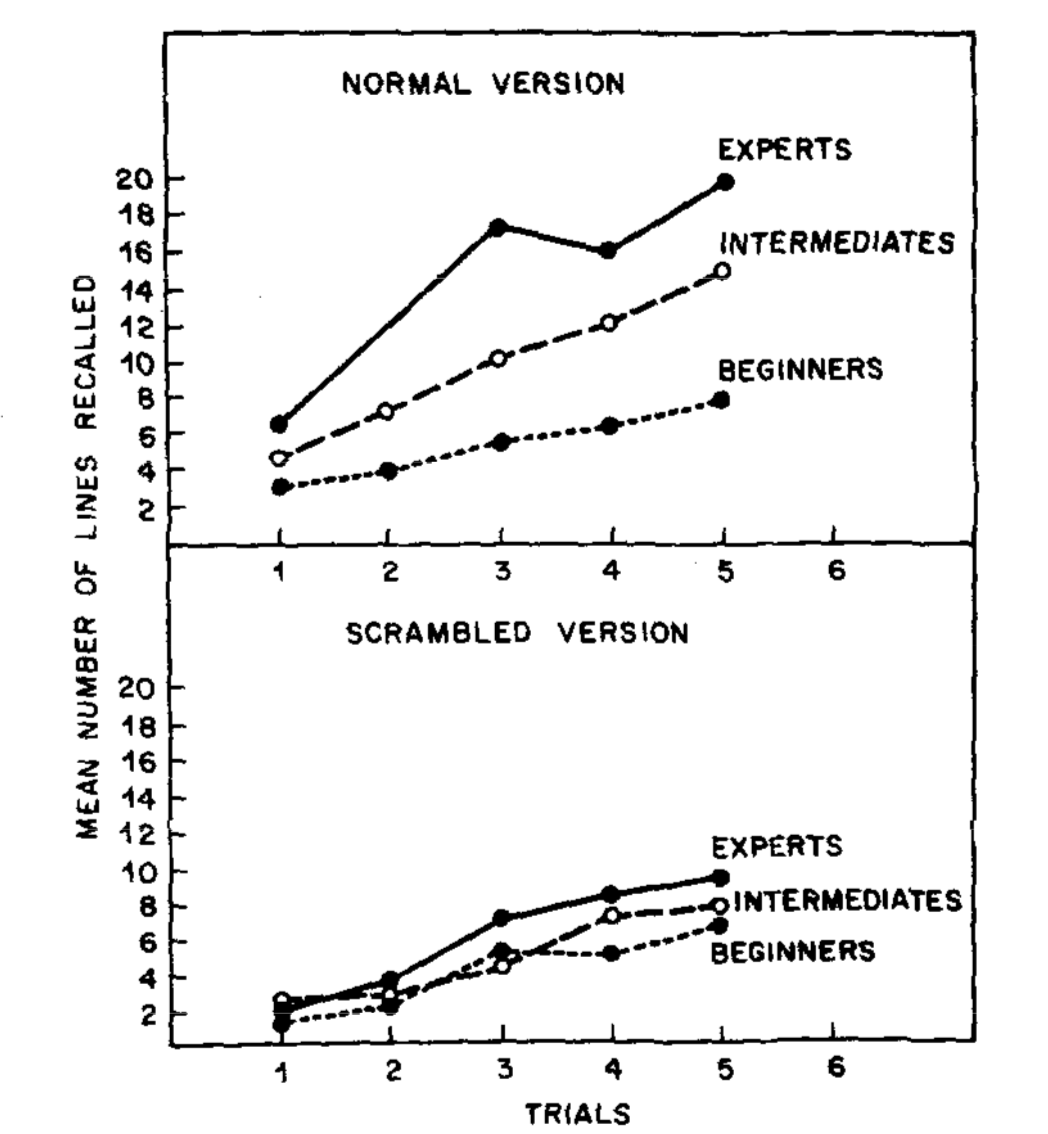
\includegraphics[width = 0.5\columnwidth]{reitmanE1.png}
\centering
\caption{Performance Differences between Experts, Intermediates and Beginners in Experiment 1 (Recalling Lines of Programs) \cite{MCKEITHEN1981307}}
\label{reitmanE1}
\end{figure}

\begin{figure}
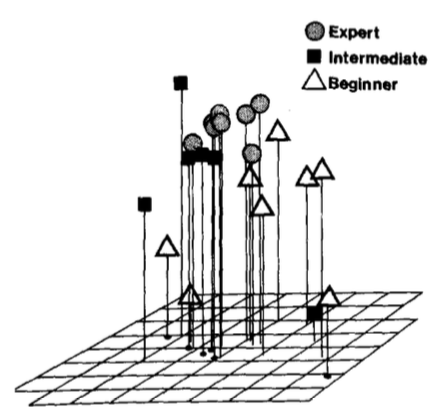
\includegraphics[width = 0.5\columnwidth]{reitmanE2.png}
\centering
\caption{Coherence between Groups of Experts, Intermediates and Beginners. Measured by Multidimensional Scaling Configuration of Distance \cite{MCKEITHEN1981307}}
\label{reitmanE2}
\end{figure}

In their second experiment, each subject was asked to organize the programming concepts in the form of hierarchical representations for keywords in computer languages such as \textsc{true, false}, \textsc{if, while} and \textsc{for}, and so on. Then they aggregated the result into a multidimensional scaling configuration for the distance between each subject. Their result suggested that experts are more cohesive to each other as a group, whose knowledge construction, i.e., the semantic representation \cite{bobrow1975representation} are particularly alike, but intermediates and beginners are not cohesive as experts (See Figure \ref{reitmanE2}).

This study has two major contributions: first, it confirmed the fact that in programming, experts are faster and precisely in processing information of computer programs which is a familiar result as in other fields. Second, it found that experts are more similar while organizing their semantic knowledge structure about programming. Moreover, in this study, expert subjects' knowledge structure have clustered a cohesive group which indicates as expertise increasing, the knowledge structure of computer programming domain will eventually be similar. 

There are a few studies later on expert characteristics and performance, such as exploring expert problem-solving strategies \cite{davies1994knowledge, koenemann1991expert}, quantifying programmer's skills \cite{stanislaw1994note}.

\subsection{Manual Expertise Location}

\textbf{McDonald and Ackerman 1998}

In early days, practitioners locate expertise to solve problems that they could not solve alone, but over manual approaches without the assistance of automated software. In 1998, McDonald and Ackerman conducted a five-month field study in a medium-sized software firm to observe practitioner's behavior in manually locating expertise within their organizational settings \cite{mcdonald1998just}.

According to their observation, three expertise \textit{identification} approaches were summarized. First, as they purposed the terminology in the paper, senior practitioners have difficulties in articulating how they know who knows a certain area, for example, a quote from their study says:

\begin{displayquote}
``You learn who's [the] most experienced in what areas. ...You just know.'' 
-Sherry
\end{displayquote}

This expertise identification approach is the \textsc{Everyday Expertise}. However, this approach is not applicable to newcomers and sometimes even to the senior member when they were unable to track everyone. The second type of expertise identification is \textsc{Historical Artifacts}. The general philosophy of this approach is finding the person who has the last authorship (change the artifact) of the artifact that related to solving the problem. However, this approach of identifying expertise is limited by the purpose or size of the change, which may falsely identify the expert.

The last approach is asking for help from an expertise concierge. In an organization, the expertise concierge is the key personnel who has very elaborated social networks and mediates many requests for information including locating expertise. Other management studies use the term of information gatekeeper \cite{allen1977managing} information mediator \cite{ehrlich1994turning} and \cite{paepcke1996information} to refer to the same role in an organization. An expertise concierge usually refers to people who were looking for information and expertise to those who may have them.

After the identification process and if there were multiple choices, the practitioners would start the process of expertise \textit{selection}. During this process, they tend to choose a person from their local social network and avoid routing to another department. Finally, the expert whom they chose to look for help might not always be the person who could offer the help due to series reasons, and this is when \textit{escalation} happens.

This study is critically important to other studies of expertise location. It purposed three main strategies to identify experts, and two of them (historical artifacts and Expertise Concierge) are directing the later studies for automated expertise identification. However, this study's research setting is a mid-size company, which did not capture the collaboration model in larger or smaller companies, especially for distributed teams. Besides, due to the age of this study and the development of knowledge sharing/transferring platforms, we argue that we need to re-evaluate our expertise location practice in the organizational settings. 

\subsection{Automated Expertise Location Techniques and Systems}

Since 2000, researchers start building systems and methods for locating the expertise based on specific needs. Notably, these studies inherit the Historical Artifacts heuristics purposed by McDonald and Ackerman \cite{mcdonald1998just}. Also, these approaches also aim to measure and quantify expertise while mining historical artifacts.

\subsubsection{Mining Historical Artifacts}

\textbf{\citeauthor{mcdonald2000expertise} 2000}

Two years later, McDonald and Ackerman published an automated expert recommendation system for solving problems in software organizations called Expertise Recommender (ER) \cite{mcdonald2000expertise}. This expertise location system attempt to decrease the workload of expertise concierge and provide alternative options. They employed their expertise locating heuristics from their previous field study, and their main strategy is based on mining the historical artifacts.

There are two basic heuristics for expertise location in ER. The first one is Change History heuristic which adopted from the ``Line 10 Rule''
from their field study \cite{mcdonald1998just}. The ER system checks for the last change of the software module in the version control system, and the developer who made the last modification would be the best candidate to ask for help.

The second heuristic is inherited from the Tech Support. It enhances the routine behavior of technical support when she faced an unfamiliar problem and starting to find a similar experience or problem in the past. Therefore, ER creates a local database for querying similar problems that happened before and associated with the person who solved them.

A user can pick the basic heuristic based on which one fits their need of the current problem, and then choose the mechanism while selecting the expert (see Figure \ref{ERUI}).

\begin{figure}
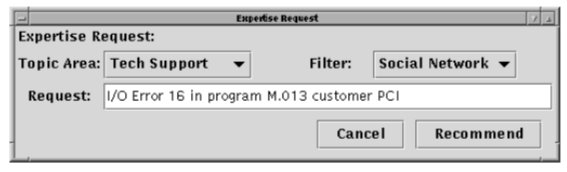
\includegraphics[width = 0.5\columnwidth]{ERUI.png}
\centering
\caption{The Expertise Request Dialog of Expertise Recommender \cite{mcdonald2000expertise}. Topic Area: Selecting the Heuristic; Filter: Strategy for Expertise Selection}
\label{ERUI}
\end{figure}

The two heuristics applied in this study are very inspiring and lead the future studies for expertise locations. Most future studies applied, integrated or combined these two heuristics for their design heuristics. For example, mine version control systems for changing history \cite{mockus2002expertise, schuler2008mining} or look for the similarity of unsolved and solved problems \cite{Anvik2006who, xu2016predicting}. This applies two data sources, changing history from the version control system and also the database of previous tech support problems. However, this system lacks a systematic evaluation or a plan on the performance of the system.

\textbf{\citeauthor{mockus2002expertise} \citeyear{mockus2002expertise}}

\citeauthor{mockus2002expertise} designed another expertise location system called \textsc{Expertise Browser} (ExB) \cite{mockus2002expertise}. Their main purpose of this study is to locate relevant expertise for collaboration in geographically distributed development. The major contribution of their work is to start quantifying a developer's expertise on specific code module based on activities and distinguish developers who have only briefly worked on a module and who have extensively worked.

In this study, they purposed a quantitative measurement of expertise without professional licensing. They defined the concept of \textit{Experience Atoms} (EAs) as the smallest unit of experience, and in practice, EAs refer to ``the smallest meaningful unit of such change,'' and the ``change'' is the direct result of a developer's activity on the product. By applying this concept, ExB summarizes a developer's expertise on changing files.

The user interface design of ExB is as follows (See Figure \ref{ExB}). For each software module, a developer would have different amounts of EAs which contribute to different levels of expertise on a specific model. In the right panel, the length of each bar on the module name represents the accumulated EAs for ``Robert Wells'' the example developer's expertise based on his activities. Intuitively, the bigger the bar represents, the higher expertise. Finally \citeauthor{mockus2002expertise} conducted a case study on distributed teams to evaluate the tool.

\begin{figure}
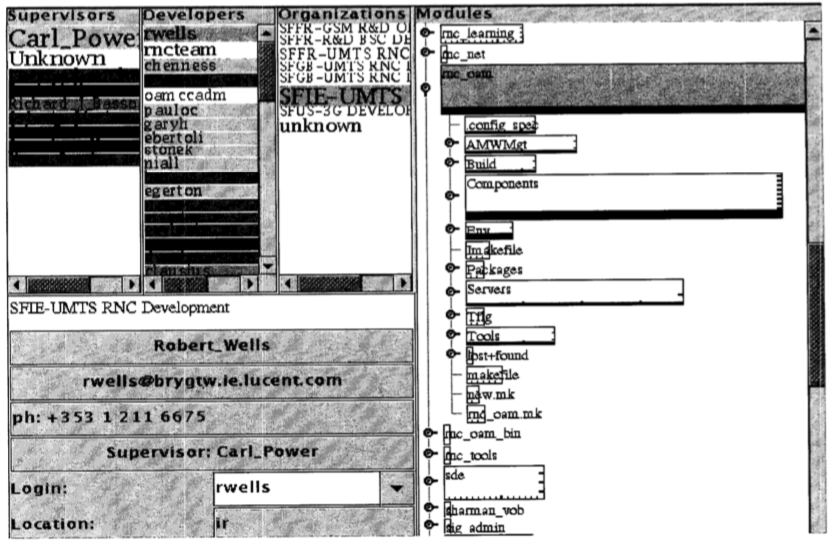
\includegraphics[width = 0.8\columnwidth]{ExB.png}
\centering
\caption{The User Interface of ExB \cite{mockus2002expertise}}
\label{ExB}
\end{figure}

Noticeably, except this study first represents the expertise in software engineering practice by the form of visualization (the area of bar charts), it gives two suggestions for future studies. First, the time of the change activity is also a critical factor to consider while building the quantitative model for expertise. In this study, the time factor is discussed to help the model the difficulty of a Modification Requests. A harder request may cause the longer time of MR interval. Though time is a critical factor in modeling and quantifying expertise, \citeauthor{mockus2002expertise} is the first to include it in the context of software engineering based on our survey \textcolor{red}{``though'' is not the right conjunction for the logic relationship you want to establish}.

In another discussion of the study, the authors were mapping experience to expertise. Though experience is not the perfect measurement for expertise, and they did not trace back to the cognitive model of expertise, their discussion provides insights on what other information can be considered in expertise measurement. Finally, they also discussed the possibility of representing a developer's expertise with visualizations. 

However, this study also has its limitation. First, it only applies the single data source, which only uses the changing log from version control system to determine the expertise. Moreover, as it is a case study, it only tested ExB's usability with participants, but it lacks user feedback or evaluation on the precision (usefulness) of the experts that ExB recommended.

\subsubsection{Expertise Concierge and Social Network Analysis}

\textbf{Nardi et al. 2002}

Earlier in 2002, information digitization has been a trend even for our contact book. As the prior work mentioned, personnel like expertise concierge plays an essential role in locating expertise under the organization setting \cite{mcdonald1998just}, but this type of role need to handle more information of other members in the team such as their contact information to find them when needs to. Thus, Nardi et al. design and implement an assistant software named ContactMap \cite{nardi2002integrating} to not only support expertise concierges to manage the contact information, and also visualize the social network of each member.

As they claimed in the paper, the major user scenarios of their tool are reminding and supporting the user. For example, reminding the user of the others' identities and connections between people in their social network, particularly the contact information of these people. In addition, ContactMap also provide \textit{awareness information} for distributed team members, such as their availability for phone calls \cite{dourish1992awareness}.

\begin{figure}
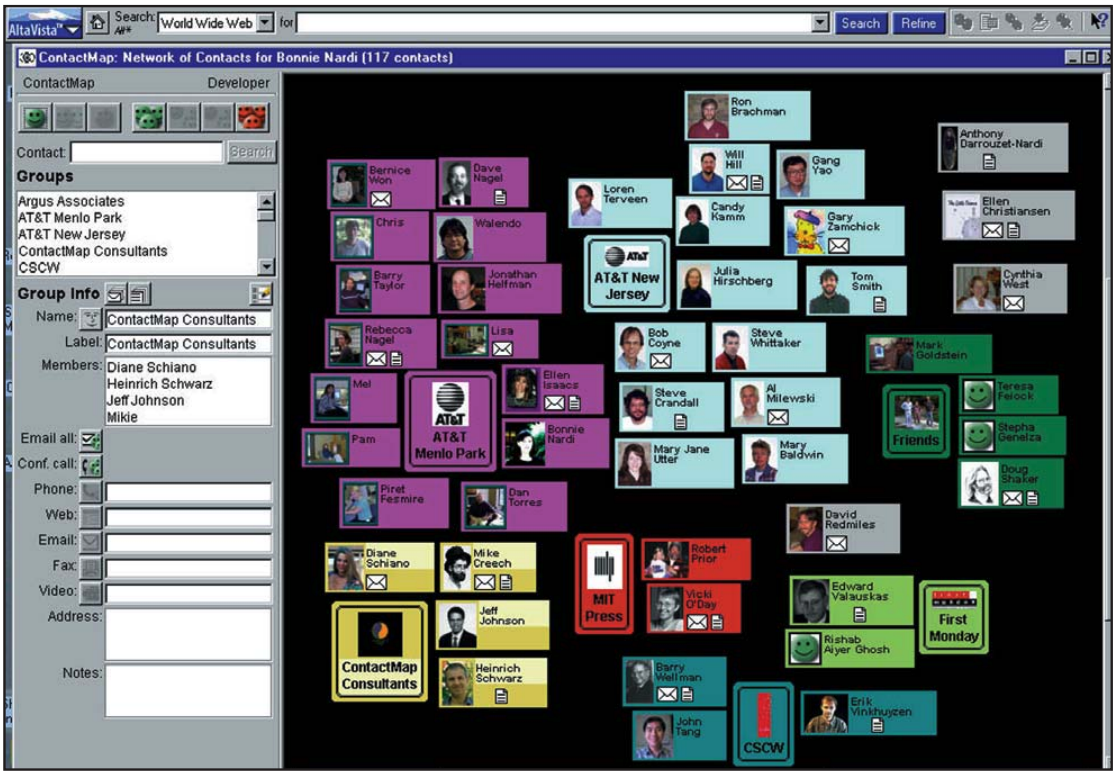
\includegraphics[width = 1\columnwidth]{ContactMap.png}
\centering
\caption{The User Interface of ContactMap \cite{nardi2002integrating}}
\label{ContactMap}
\end{figure}

This is an exploratory study of leveraging the social network of team members and support collaboration and communication. Moreover, they were also the pioneers in visualizing social networks  In the future, they plan to address more detailed research questions such as how people use this tool (evaluation of this work)?; How to support task-specific network?; Whether to hide peripheral members of the task in ContactMap and so on. They lead the discussion on this topic.

\textbf{Lin et al. 2009}

As a follow-up study on the social network analysis, Lin et al. design a social network data mining tool called Smallblue \cite{lin2009smallblue}.

In this work, they pushed the research of social network one step further by analyzing the social network and generating location of the key persons in it. They identify the key people, "Key Hubs" in the network through graph analysis such as locating structural holes. Besides the identification function, they also provide \textit{awareness information} in their tool, such as displaying the geographical information for each team member.

\begin{figure}
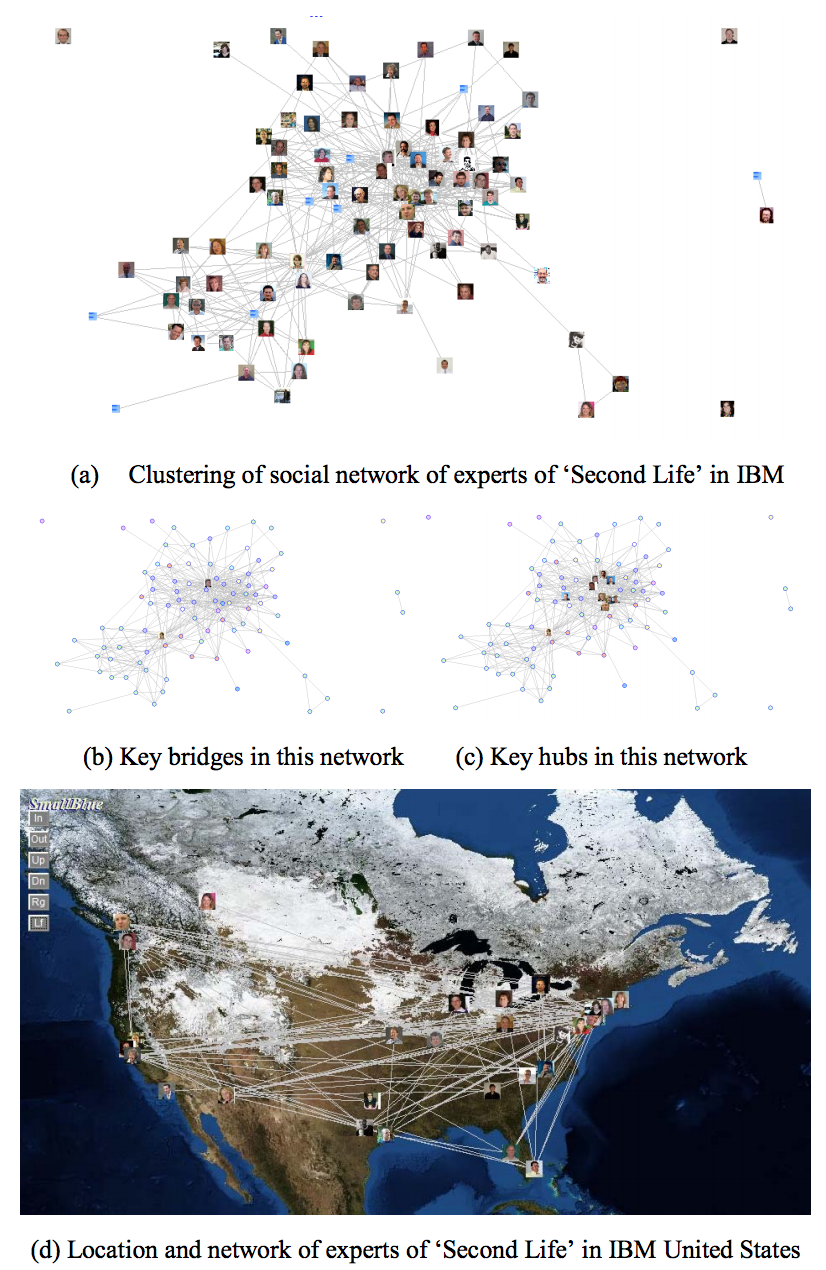
\includegraphics[width = 0.6\columnwidth]{smallblue.png}
\centering
\caption{The User Interface of Social Network in Smallblue \cite{lin2009smallblue}}
\label{Smallblue}
\end{figure}

Comparing with previous work, their visualization of a social network is more detailed in different perspectives and provide richer information on an individual team member. Moreover, it gives more personal information which is beyond contact information only. This tool combines the social network attribute and expertise. Finally, it was an online web tool\footnote{http://smallblue.research.ibm.com} which is maintained by IBM, though it is no longer maintained and offline now.

\section{Open Source and Knowledge Sharing Site}

\subsection{Empower Open Source}

In 1983, Richard Stallman launched the GNU Project with free source code sharing online. Later in 1991, Linux was released by Linus Torvalds with the license for freely modifiable source code, which significantly promoted the movement of open source software. Until 2005, the most popular decentralized version control system was created, and three years later, GitHub was launched, which fundamentally changed the development process and collaboration approach for open source projects. Later in the 2010s, studies also suggest that open source contribution is also a factor to consider in the software developer hiring process. The publicity afforded by these open source projects, dramatically promotes the development of software engineering research, particularly for empirical software engineering studies. Moreover, researchers can utilize valuable public historical data for locating expertise. 

\textbf{Anvik et al. 2006}

As the emergence of machine learning technologies in software engineering, this study by Anvik et al. started to assigning bug reports to developers based on their historical activities. The main purpose of this study is to alleviate the burden of managing bug report repository in large open source development teams.

As the first study to locate expertise by using machine learning techniques, their approach trains the machine learning algorithm based on the historical experience of a developer. Their algorithm models the types of the bug that a developer had solved before, and then based on the type of the bug report which needs to be assigned which predicts developers performance on an unsolved bug. Finally, it generates a list of developers who are considered as experts on solving such a bug. To empirically validate their tool, they analyze 3,426 bug reports for Eclipse.

To characterizing bug reports, they convert text in summary and description into feature vectors which can be trained by machine learning. They applied a set of heuristics to identify the expertise based on the bug resolving history. The basic four types of which they provided in the paper are:

\begin{itemize}
\item \textit{If a report is resolved as FIXED, it was fixed by whoever submitted the last approved patch. The person who solved it in the last approved patch has the expertise.}

\item \textit{If a report is resolved as FIXED, it was fixed by whoever marked the report as resolved. The person who marked it as resolved has the expertise.}

\item \textit{If a report is resolved as DUPLICATE, it was resolved by whoever resolved the report of which this report is a duplicate. The person who resolved the report has the expertise.}

\item \textit{If a report is resolved as WORKSFORME, it was marked by the triager \textcolor{red}{trigger?}, and it is unknown which developer would have been assigned the report. The report is thus labeled as unclassifiable at the moment.}
\end{itemize}

In their approach, they applied a systematic method to evaluate the recommendation of the bug report resolving expertise based on the principle information retrieval technique, precision, and recall. They regard expertise location process as a process of information retrieval, and the query is an unsolved bug report which would be used for search experts. However, the result is not promising at that time. They have only achieved 57\% and 64\% of precision for two projects, and recall is not over 10\% for either project. Noticeably, the ground truth for evaluation on this machine learning technique is based on cross-validation. Therefore, the developer who is identified as the expert for a bug report may not carry the expected expertise.

Though this study's result does not look so great regarding percentage numbers (especially comparing to the state-of-art bug report assignment techniques), they lead a trend of research in software engineering by applying machine learning techniques to locate expertise, and also utilize the extensive data provided in online open source repositories.

\textbf{Schuler and Zimmermann 2008}

In this study, Schuler and Zimmermann refined the model of expertise on code artifacts purposed in previous studies, especially the quantitative expertise model purposed by Audris and Hebsleb in 2002 \cite{mockus2002expertise}. In addition to quantifying the expertise based on a developer's modification on the code artifact, they also introduce the concept of \textit{usage expertise} which is more straightforward to collect.

The usage expertise is the knowledge that developers would also accumulate while using other functionality such as calling APIs, which they did not implement. They argue that while calling (using) methods, developers might not be aware of implementation details, but these developers would gain expertise on how to use a method and when a method can be used.

Including refining the model of expertise on code artifacts, this study also mentioned the application of creating an expertise profile for a developer. However, due to the limitation of mining techniques, it only provides low-level information on a developer's expertise, and still needs human interpretation to refine high-level expertise summary. Moreover, the social network of developers is hard to extract information (see Figure \ref{usage}).

\begin{figure}
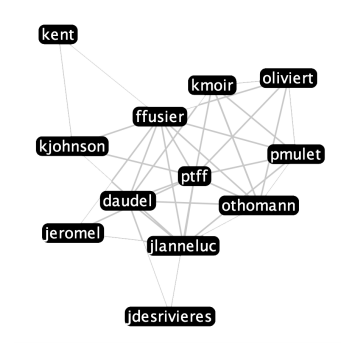
\includegraphics[width = 0.4\columnwidth]{usageExpertise.png}
\centering
\caption{An Example of Developers Usage Expertise in Their Social Network. These Developers Mostly Use the the JDT Compiler \cite{schuler2008mining}}
\label{usage}
\end{figure}

This study did not provide an evaluation or plan for your methods. However, their contribution on the quantitative model of considering what is missing at that stage is valuable, and it leads other studies to utilize the enormous data source of version control archives fully.
%rephrase it later.

\textbf{Fritz et al. 2010, 2014}

In their journal publication in 2014, Frtiz et al. summarized their work modeling expertise for code authorship and interaction. They purpose a model to capture the developer's expertise on source code element, \textit{Degree-of-knowledge}(DOK). This model utilizes the IDE to track developer's interaction with the code, and they empirically identified their results on two sites (two software development teams).

This study introduces the DOK model which represents developer's familiarity with code element. In their model, DOK is the combination of degree of authorship and degree of interest:

\begin{equation}
DOK = \alpha * DOA + \beta * DOI
\label{DOK}
\end{equation}

Particularly, the degree of authorship data is mined from version control achieves. Defined in the paper,  the degree of authorship data contains three factors (\textit{first authorship, deliveries, and acceptances}). Mylyn (was Mylar) \cite{kersten2005mylar}, an IDE plugin in Eclipse collects them as well as the degree of interaction data. The degree of interest of a code element is accumulated with each interaction the developer had with it, for example, clicking or selecting a variable name rather than editing it.

For determining the weightings, $\alpha$ and $\beta$ in the Equation \ref{DOK}, they collected the data from developers in the team, and let developer themselves to rate their knowledge about code elements as the ground truth of expertise, and then apply linear regression to decide weights in Equation \ref{DOK}.

\textbf{Servant and Jones 2012}

This paper introduces a technique called \textsc{WhoseFault} which is automated to choose expert developers to fix execution faults reflected by test cases. By applying this approach, the faulty test case can be assigned to the developer who may have the expertise to resolve the failure. Second, similar to the previous work of the second author, it provides a diagnosis of where the lines of code may cause the fault.

\begin{figure}
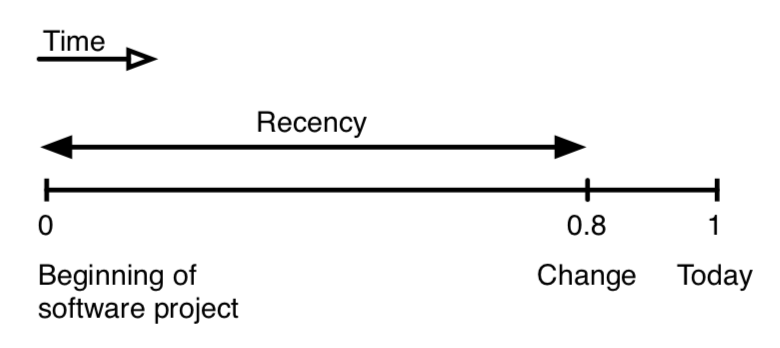
\includegraphics[width = 0.5\columnwidth]{recency.png}
\centering
\caption{The approach of calculating \textit{recency} based on the time of starting at the beginning of software project \cite{servant2012whosefault}}
\label{recency}
\end{figure}

Their approach does not only leverages the version control system to gather data but also utilizes the test cases and their execution results to complimentary the expertise model. This technique extracts the history of source code with its test cases execution result to locate the fault within the source code. It applied the same technique from their previous study \textsc{TARANTULA} to automatically local buggy code by assigning the \textit{suspiciousness} score to each line of the code \cite{jones2002visualization}. In this study, they moved one step forward to assign execution fault to developers with expertise or responsibility based on the suspicious code.

Besides \textsc{WhoseFault}'s implications on reducing bug reports generation as they claimed in the paper, this study also contributed to expertise location techniques, particularly on interpret and evaluate the quality of developer's previous working experience. Another critical contribution is that in their quantitative expertise model, they specifically consider the time factor and introduce the \textit{recency} in expertise calculation see Figure \ref{recency}. Though early study \cite{mockus2002expertise} has mentioned time would be a factor donates to the expertise measurement, but their emphasis was measurement on the difficulty of the task. 

In their evaluation, besides comparing to other similar expertise location techniques, their ground truth of expert for fixing the fault is based on the actual developer who performed the bug fixing action later. Therefore, the developer who fixed the bug is the expert. Though this method has its limitation which raises challenges such as the bug fixer may not be the best developer with the expertise, and so on. This method improves evaluation strategies, and it refers to the philosophy of evaluation approach for machine learning techniques. 

\subsection{Emergent Expert for Open Source}

\textbf{Yu et al. 2016}

The pull-request model is a widely adopted by distributed teams, especially open source ones. However, conventionally a project owner performed manually assign the developer to review the contribution, or the owner would review by herself. This manual process is time-consuming and ineffective, and it usually overburdens some team members. As a part of expertise location research, determining several best candidates for the code reviewing task is an emergent need as open source communities getting popular in software production.

In Yu's study in 2016, they purposed a method for pull-request code reviewer assignment, which automatically recommends the expert for reviewing the source code contributed in pull-request, they identification and selection procedure grounded by previous development history. Particularly, they combine their expertise factors and common interests of developers into their expertise location model.

IN addition to an experience based on the expertise model, their rationale of analyzing social interaction is based on the formation of pull-request review commit on GitHub. Since on GitHub, core team members for a software repository may not always be able or available to review the pull-request, and also because GitHub is \textit{social coding} site, outsourcing the expertise from external reviewers is usual, and they play critical roles in helping and affecting the code team members while determining whether to approve the pull-request \cite{tsay2014let}. Therefore, the interaction history of the external reviewers by comments shows their interests towards the repository, and also indirectly reflects their knowledge and expertise in the repository.

By combining this social interaction data to the experience based expertise model, they leverage the social character of the open source platforms. Noticeably, they conduct a mix method approach to evaluate their approaches. Like other recommend systems before, they adopted precision and recall to assess the performance. Moreover, they conduct a qualitative study to deeply explore the benefit of their expertise location approach by combining social interaction. Their results suggest that technical keyword in communication traces is the most relevant factor in determining the expertise of a developer to the project, and for a project has most reviews are insiders, a developer who becomes a \textit{dominant reviewer} usually leaves her communication traces in most of the pull-request. For this type of collaboration mode, one repository only has a few dominant reviewers.

\textbf{Costa et al., 2016}

Besides the pull-request model, merging is another important collaboration practice, as parallel development is beneficial to manage time to release the product either in open source communities or commercial development. However, merging is not an easy task to perform as it requires complex expertise in resolving conflicts \cite{costa2016tipmerge}. 

Current techniques and tools only detect straightforward and direct conflict such as textual conflict. However, these tools are not able to realize complex cases such as unseen dependency modifications \cite{shihab2012effect}. Therefore, it is very typical to assign a developer to manually resolve the conflict or confirm if the merge is free from potential conflicts. However, it is not clear to find the appropriate developer or locate a few experts to perform the merge action.

\begin{figure}
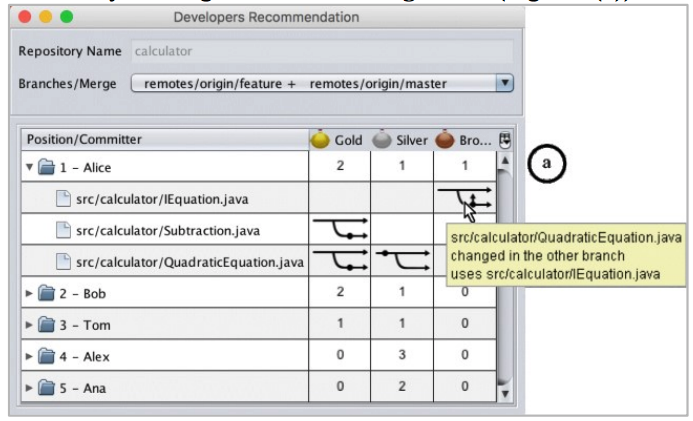
\includegraphics[width = 0.5\columnwidth]{TipMerge.png}
\centering
\caption{User Interface of Showing Rankings of Developers for Performing Merge in TipMerge \cite{costa2016tipmerge}}
\label{TipMerge}
\end{figure}

In their study, they purposed an automated approach called \textsc{TIPMerge}, a novel tool which identifies a list of developers as the best candidates to perform the merge action. Similar to other expertise location systems and approaches, it determines the expertise for performing the merge based on developer's previous experience with the branch and the project, particularly the interactions with key files for the merge and their dependencies (See Figure \ref{TipMerge}).

Finally, they evaluate their system based on a mix-method approach similar to \cite{yu2016reviewer}. They not only quantitatively compared their result with conventional methods, but also conduct a qualitative study by interviewing team members for two projects. As they summarized, there are couple reasons other than previous experience to decide a merger, such as, ``Line 10 Rule'' for merge (the developer who made the last commit would help the merge); knowledge on the trick part of the code artifact; personal preference.

\subsection{Emergence of Knowledge Sharing Sites}

Effective knowledge sharing platform has been emergent since the late 2000s (Stackoverflow launched in 2008). The free knowledge crowdsourcing practice has changed the way how developers get basic knowledge on programming questions. It was great idea and effort for Stackoverflow to organize the documents for each programming language and API, but the company has to end the project due to its enormous effort in management and low profit for return\footnote{Stackoverflow Meta, Sunsetting Documentation: https://meta.stackoverflow.com/questions/354217/sunsetting-documentation}. However, a complete documentation or code examples is necessary and affordable for private knowledge resources such as knowledge sharing repository for private companies and commercial project, for example, Software Engineer from Facebook, Satish Chandra introduced the internal code repository of Facebook on 2018 ISR research Forum at University of California, Irvine\footnote{https://isr.uci.edu/content/2018-isr-research-forum}. Properly utilize the knowledge sharing site to locate expertise is critical but the current research has been struggling with the extracting relevant information partially due to the ambiguity of natural language. Research on knowledge sharing sites is still in the beginning and building infrastructure phase.

\textbf{Hanrahan et al. 2012}

It is intuitive that a person with high expertise on the domain could answer hard related questions in software engineering, and novices in the domain could not. However, the difficulty of questions is hard to model. In this study, Hanrahan et al. employ a straightforward method to model the difficulty of a question on Stackoverflow by calculating the time duration between the problem is posted and the accepted answer is posted.

It is not a brand new idea to model the difficulty and expertise. Earlier in the study of \cite{mockus2002expertise}, they have already discussed the time issue of a task in software engineering, such as a hard request or bug would take more time to complete since it was issued. However, they did not include the time factor in their quantitative expertise model. In this study, the authors only consider the solving time as a factor, but they missed the other factors contributing to the solving time such as the popularity of the topic, question asker's representation of the question, and special cases such as adjust the question by other comments \textcolor{red}{hard to understand}. However, they provide an initial approach to model the expertise in questions through time factor.

\textbf{Xu et al. 2016}

Due to the ambiguity of natural language, and different representation may refer to the same semantic meaning, questions on Stackoverflow may be repeated or high related to each other. Removing the redundancy and simplifying the variations are critical for modeling the users' expertise and avoid information overload for knowledge providers and receivers on knowledge sharing sites. Unfortunately, Stackoverflow is not able to manage its enormous knowledge base like Wikipedia\footnote{https://www.wikipedia.org/} which links keywords, i.e., knowledge unit, to its own explanations. As the failure of Stackoverflow Documentation which is due to the nature of programming language, the complicity of programming knowledge unit is not affordable to human labor to classify.

Therefore, Xu et al. employ the convolutional neural network to model the knowledge unit in questions and answers for expertise. Through the techniques and approach described in their study, they can cluster different word representations into different high-level categories \ref{knowledgeUnit}. Besides, they also use precision and recall as the primary evaluation metrics for their approach.

\begin{figure}
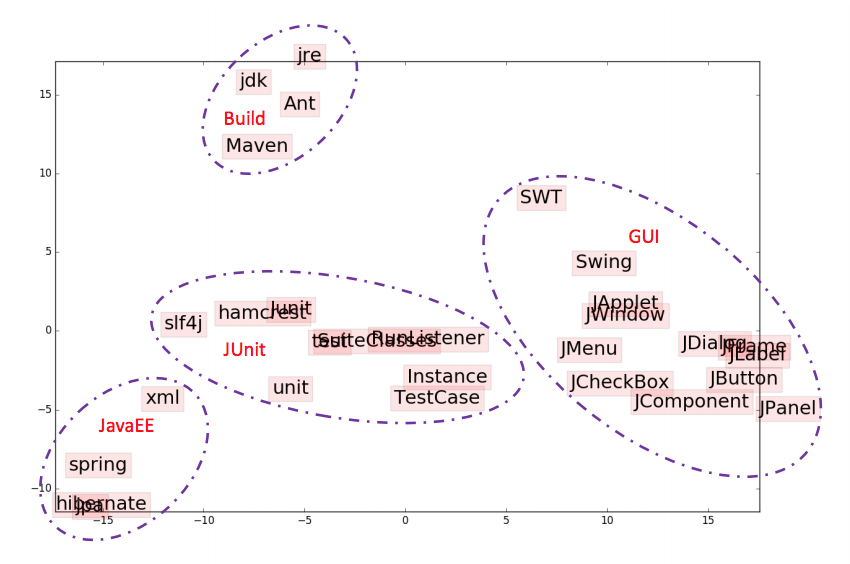
\includegraphics[width = 0.5\columnwidth]{KnowledgeUnit.png}
\centering
\caption{Word Representations Embedding Examples \cite{xu2016predicting}}
\label{knowledgeUnit}
\end{figure}

Based on their study, it is possible to manage the knowledge unit, defined in their study, and link them as Wikipedia. It enhances the usability of the site and also easier to mine a knowledge unit related expertise for developers which is at a higher level than ``tag'' in Stackoverflow.

\section{Multiplatform Data Aggregation}

\textbf{Sarma et al. 2016}

As the emerging of community-based knowledge sharing platform, e.g., Stackoveflow and open source platform, e.g., GitHub, it is necessary to monitor and aggregate a developer's activities all over the internet for precisely measuring her expertise in software engineering for both ``soft'' social skills and also technical skills.

Therefore, Sarma et al. design and implement a visualization tool, \textsc{Visual Resume} to include a developer's activities over the internet. Notably, other than the amount of the contribution for a developer over his career (bar charts in the middle of each card in Figure \ref{vr}), it also provides quality indicators of their contribution such as whether a pull-request is accepted and whether their commit passed the test cases provided in the repository. Besides, it employs a card-based user interface to allow easy comparison between developers, and mainly they design this tool to extract expertise from historical contributions for hiring purpose.

\begin{figure}
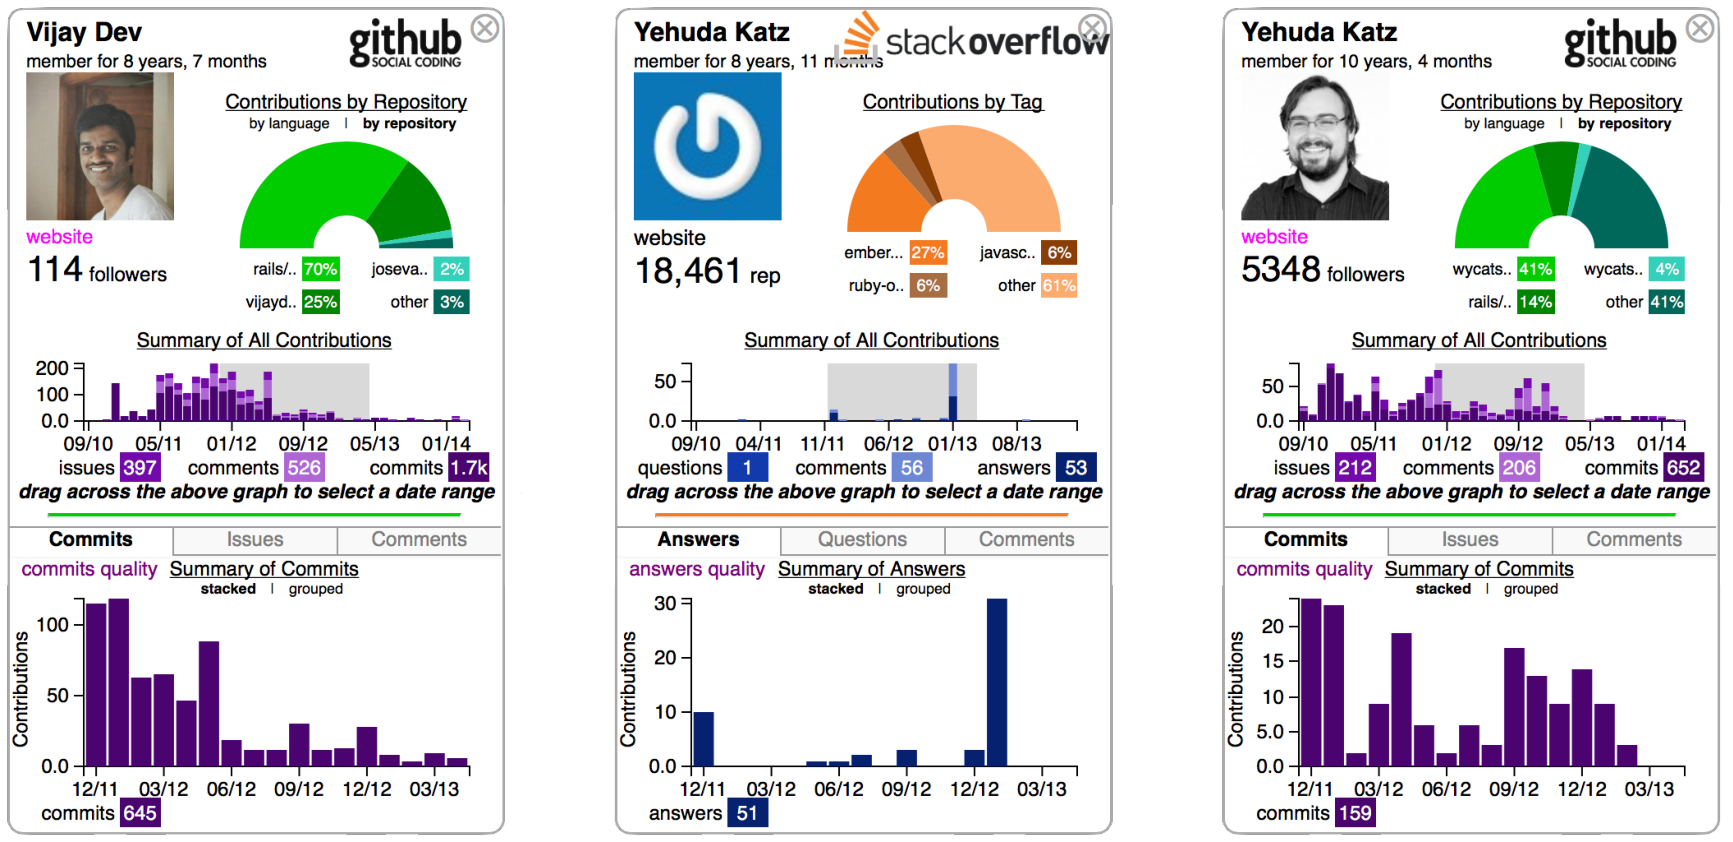
\includegraphics[width = 0.8\columnwidth]{vr.pdf}
\centering
\caption{The Card Based User Interface for Comparing Expertise in the Hiring Procedure \cite{hiring2016sarma}}
\label{vr}
\end{figure}

As for evaluation, they conduct the interview based usability test with management level of personnel from industry, and let participants either use the web portals of developer's profile or use \textsc{Visual Resume} to evaluate job candidates based on job description, and then select best candidates for the job. Particularly, other than finding \textsc{Visual Resume} is helping participants in making their decisions, participants also mentioned that the qualitative interview phase is still necessary as a part of hiring new employees.

\section{Findings Summary}

In this section, we summarize the major findings from our survey review. First, we present a historical view of expertise location systems and approaches in the development of software engineering. Further, we argue that there are some limitations to the current trend of expertise location systems, especially on their dataset to determine the expertise and evaluation methods for the system. Finally, we provide some suggestions based on the current research status.

\subsection{Evolution of Automated Techniques: From Locating Expertise of ``Playing Chess'' to ``Moving Pawn''}

In this study, we reviewed the studies of expertise location in a historical perspective. We summarize the development of expertise location studies in the figure (see Figure \ref{history}).

\begin{sidewaysfigure}[ht]
    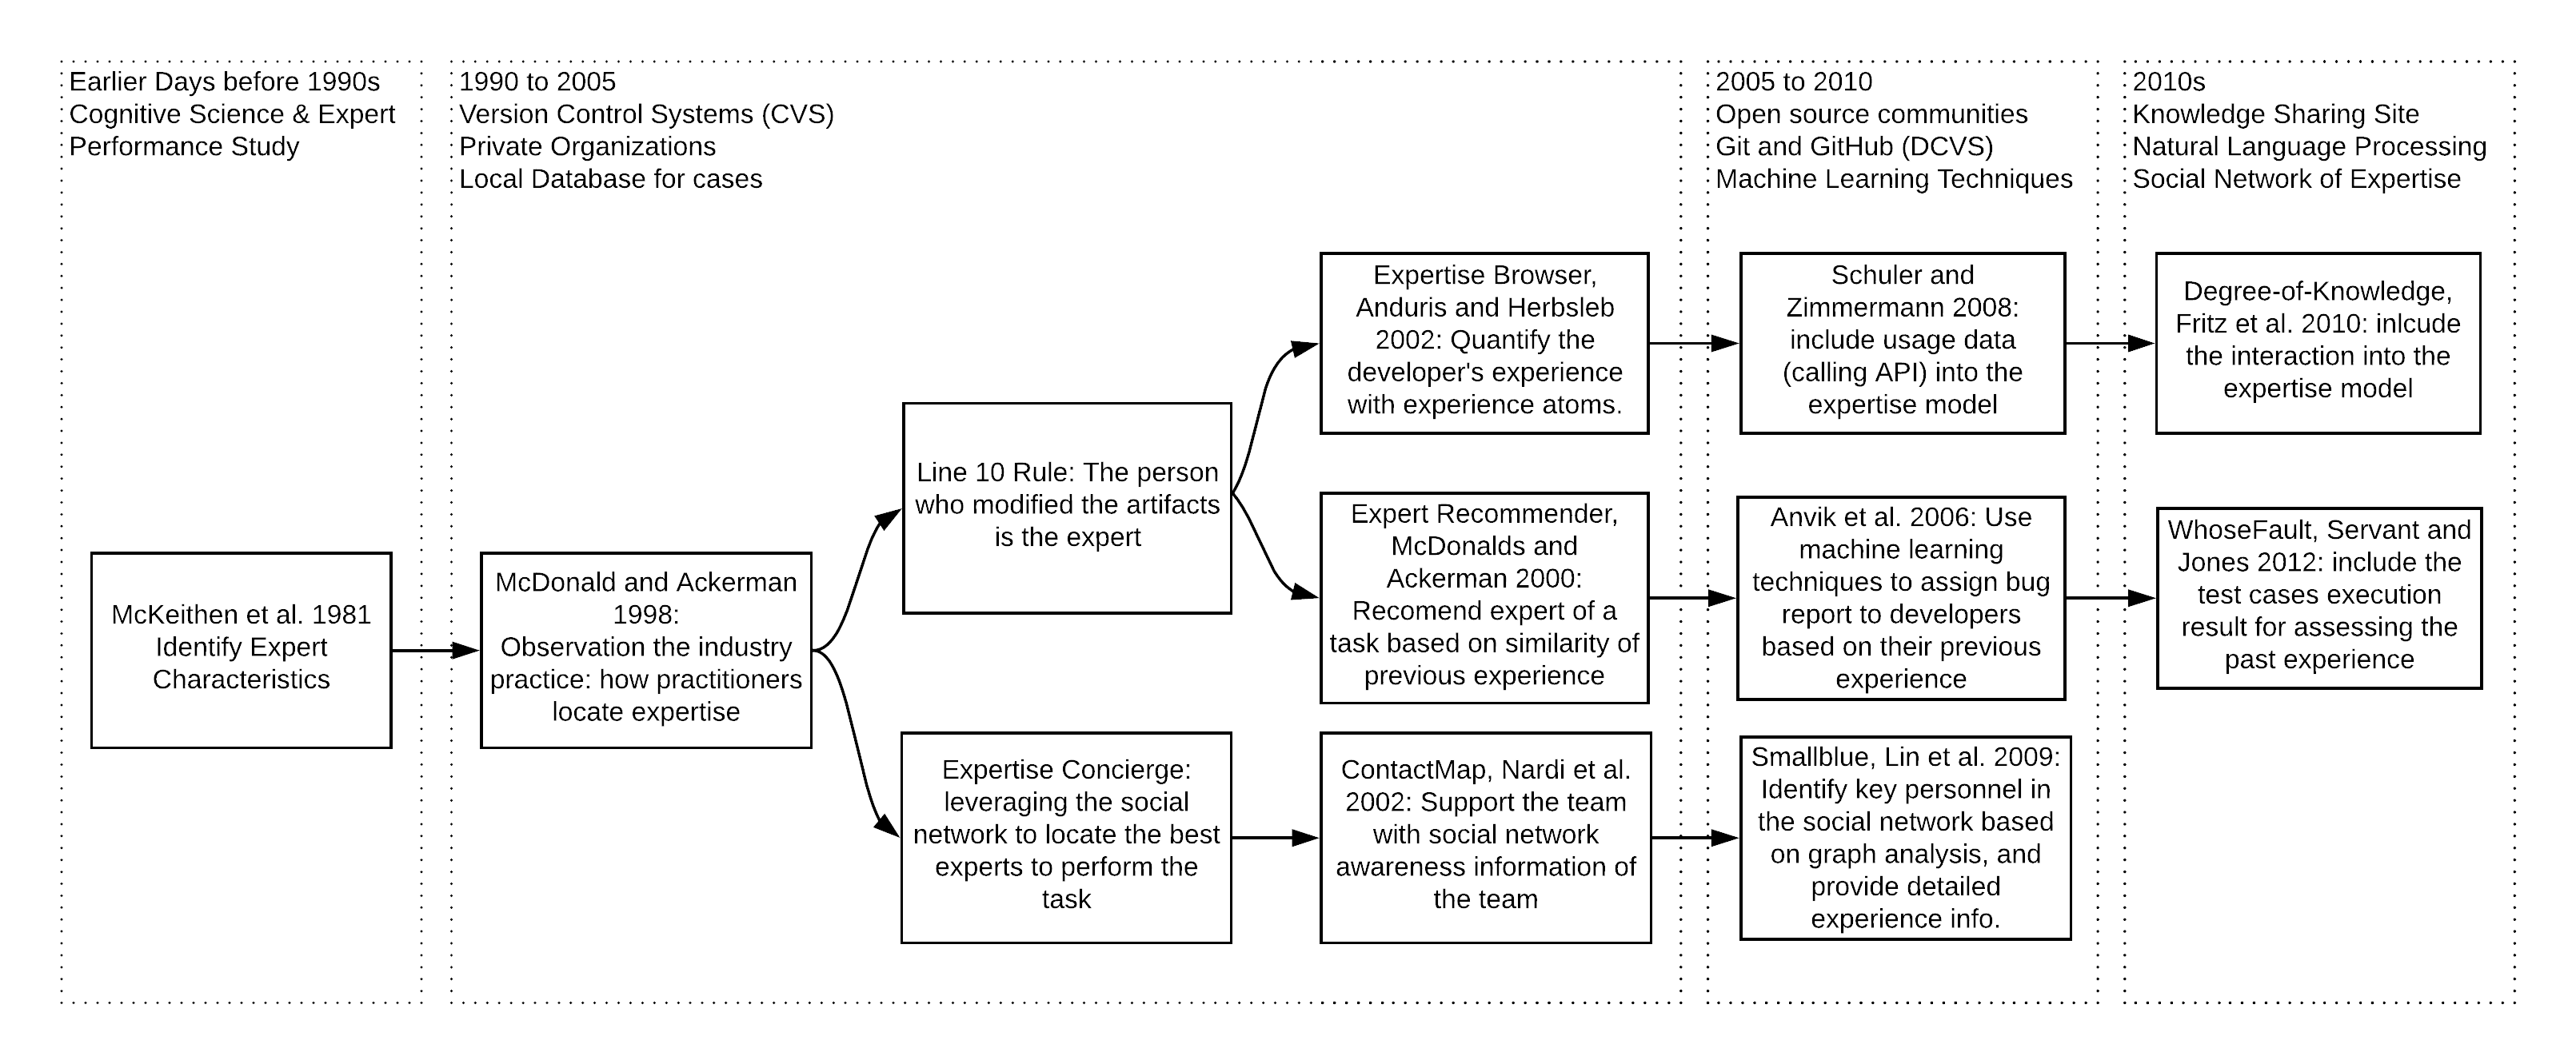
\includegraphics[width=\textwidth]{History.png}
    \caption{The Development History of Research in Expertise Location Systems and Approaches}
    \label{history}
\end{sidewaysfigure}

Early expertise research, researchers were discovering the characteristics of experts and masters, and they found experts perform better in their expertise domain mainly due to their higher information processing abilities, and this conclusion has been confirmed by a few studies in software engineering which found senior expert programmers can also process information of code faster and more precise.

Since the field study by McDonald and Ackerman in 1998 \cite{mcdonald1998just}, they set up the heuristics for expertise location systems and approaches later, mostly mining the historical artifacts or through expertise concierge. By studying our paper repository, we found automated expertise location techniques inherit and employ these two heuristics when manually locating experts. However, to the best of our knowledge, the research of expertise concierge has mostly vanished since IBM Smallblue \cite{lin2009smallblue}. On the other hand, research mines historical artifacts go to a direction of similar granularity of expertise. Automated expertise location research has a trend of going to the micro level of tasks, for example, recent research \cite{yu2016reviewer, costa2016tipmerge} focus on microtasks in open source software engineering such as merging different branches. We found the trend of going to a micro level of expertise is necessary for performing a specific low-level task (``\textit{moving pawn}''). However, when stakeholders need to perform high-level task such as locating best candidate for training and hiring new employers among candidates which require (``\textit{playing chess}''), low level expertise information closely related to programming task itself such as expertise in calling APIs is usually not intuitive to help decide the best candidates for an engineer job.

\subsection{Expertise and Time}

Only very few studies consider that expertise is not a static attribute of developers. Sarma et al. found the fact from their user study that practitioners in hiring committees of programming jobs decide a job candidate's expertise for programming task and their availability partial based on their recent activities \cite{hiring2016sarma}. Servant and Jones also consider recency as a factor in their statistical model of measuring expertise for dealing with fault, i.e., with the same amount of contribution if a developer submitted the code more recently then this developer has the higher expertise in the related issue. Early studies by \cite{mockus2002expertise} also mentioned the time issue in measuring expertise, but they intend to use the time as a measure for quantifying the difficulties and expertise required to perform the task which is under another topic. We argue that developers' expertise is continuously accumulating and diminishing. It is non-trivial to consider the time factor when measuring expertise.

\subsection{Evaluation of Expertise Location Approaches and Systems}

In this study, we found a variety of evaluation methods for expertise location approaches, but generally, previous researchers were struggling in evaluating the expertise location research and especially building the ground truth of their studies.

Earlier expertise location research usually conduct an usability test with practitioners \cite{mockus2002expertise} or even without an evaluation phase or plan \cite{nardi2002integrating, mcdonald2000expertise}. Later, \textit{Precision and Recall} becomes one of the most popular evaluation approaches to assess the effectiveness of an expertise location tool \cite{Anvik2006who, xu2016predicting, yu2016reviewer}. However, it is still hard for them to build ground truth for the result of expertise location, and cross-validation is the general solution. For example, slicing the history at a certain point of time, and uses the data before to create a reference for expertise, and then employ later data (e.g., the developer who fixed the bug) as ground truth. Though there are more factors lies between the best candidate for the task and the person who performs the task such as availability or training reasons. The complex environment and significant turnover of developers in open source projects entail more reasons of the person who performs the task in reality \textcolor{red}{unclear sentence}. However, employing the historical data is the most generic method for building the ground truth of expertise.

Due to the limitations in the evaluation of these studies, recent studies adopt a mix-method approach to build and validate the ground truth for evaluating expertise location techniques \cite{yu2016reviewer, costa2016tipmerge, xu2016predicting}. With a detailed qualitative study, these studies may be able to reveal precise expertise sharing network inside actual teams, but since the cost of these studies, researchers are not able to provide such detailed qualitative study for various environment.

\subsection{Call for a Field Study}

The last field study for locating expertise in the domain of software engineering is conducted at 1998 \cite{mcdonald1998just}, when software organizations were all private without open source communities, and also developers activities and behaviors records were stored locally inside the company. Therefore the earlier expertise location practice focus on the private data sources, including organization staff who played as key roles like expertise concierges.

However, it has been 20 years since the early field study, and both the techniques support and collaboration practice have been completely changed. The emerging techniques like machine learning techniques to support software engineering activities, natural language processing techniques to classify textual description, are significantly improving the experience of software development. New collaboration practice such as widely using the DVCS in parallel programming to save time to the market. Moreover, the internal and public knowledge sharing site is also changing the strategy of developers while transferring expertise and solving problems.

We argue that there is a need for questionnaire surveys, observations, or field studies to explore the expertise location approaches and heuristics in modern software engineering practice. Moreover, there is a need to explore the role of open source communities, knowledge sharing sites, professional social network and automated expertise location tools in the model software development. The future study shall be conducted for different purposes of expertise location studies such as hiring, training, and performing tasks.